\documentclass[a4paper,12pt]{article}

\usepackage{amsmath,amssymb,amsthm,tikz}
\usetikzlibrary{calc,arrows.meta}
\usepackage[margin=20mm]{geometry}

\setlength{\parindent}{0pt}
\setlength{\columnsep}{1cm}

\begin{document}

\twocolumn

\thispagestyle{empty}

\begin{center}
{\Large Sample Assignment 6}\\
{\Large Discussed on 2020-10-26,}\\
{\em Not graded} 
\end{center}

\noindent


\vspace{10pt}
{\bf Question 1 (Minimum and Maximum Heap Invariant.}\\
{\bf (A)} Assume that heap is implemented as a
$0$-based array (the root element is $H[0]$), and the
heap supports $\text{\sc DeleteMin(H)}$ operation that 
should remove the minimum element (and return the heap into 
consistent state).\\
({\em Note.} A consistent state in such a heap means that 
the key in parent does not exceed keys in left and right child.)\\
Find, if the heap property holds in the following array:
$$H[0]=6, 17, 25, 20, 15, 26, 30, 22, 33, 31, 20.$$
If it is not satisfied, find, which two keys
you could swap in this array so that the heap property is satisfied again.
Write the correct sequence of array $H$. 


\vspace{10pt}
{\bf (B)} Assume that heap is implemented as a
$0$-based array (the root element is $H[0]$), and the
heap supports $\text{\sc DeleteMax(H)}$ operation that 
should remove the maximum element.\\
If the heap does not satisfy invariant (in a consistent
max-heap, every parent 
should always be at least as big as both children), then show how to 
swap two nodes to make it correct.\\
$$96, 67, 94, 10, 67, 68, 69,  9, 10, 11, 50, 67.$$


\vspace{20pt}
{\bf Question 2 (Insert into a Min-Heap.}\\
Show what is the final state of a heap after you insert number $6$ into 
the following ``minimum-heap'' (represented as a zero-based array): 
$$9, 18, 28, 23, 20, 29, 33, 25, 36, 34, 23.$$


\vspace{20pt}
{\bf Question 3 (Delete maximum from a Max-Heap.}\\
Show what is the final state of a heap after you remove the maximum from
the following heap (represented as a zero-based array): 
$$96, 67, 94, 10, 67, 68, 69,  9, 10, 11, 50, 67.$$


\newpage


\vspace{10pt}
{\bf Question 1.} {\bf (A)} Answer:\\
$6, \textcolor{red}{15}, 25, 20, \textcolor{red}{17}, 26, 30, 22, 33, 31, 20.$

To see, which numbers we need to swap, we draw the original 
array as a tree (and verify the heap invariant). 

\begin{figure}[!htb]
\center{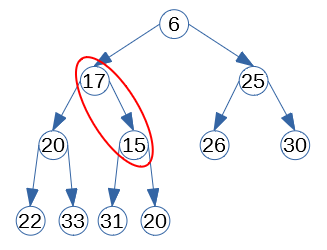
\includegraphics[width=3in]{assignment06-heaps/unsorted-heap.png}}
\caption{\label{fig:unsorted-heap} Violated min-heap invariant.}
\end{figure}

{\bf (B)} Answer:\\
$96, 67, 94, 10, 67, 68, 69,  9, 10, 11, 50, 67.$

This tree is already correct (regarding the max-heap property). 

\end{document}



